\documentclass[xcolor=dvipsnames]{beamer}

\usepackage{graphicx,subfigure,url}

\def\bfx{\mathbf{x}}
\def\bbP{\mathbb{P}}
\def\cH{\mathcal{H}}
\def\cY{\mathcal{Y}}
\def\cL{\mathcal{L}}

% example themes
\usetheme{Frankfurt}
\usecolortheme{seahorse}
\usecolortheme{rose}

% put page numbers
% \setbeamertemplate{footline}[frame number]{}
% remove navigation symbols
% \setbeamertemplate{navigation symbols}{}

\AtBeginSection[]
{
  \begin{frame}
    \frametitle{Table of Contents}
    \tableofcontents[currentsection]
  \end{frame}
}

\title{Graves 2013, ``Generating Sequences with Recurrent Neural Networks''}
\author{Johannes Bausch and Jack Kamm}
\date{14 November 2017}

\begin{document}

\frame[plain]{\titlepage}

\begin{frame}[plain]{Outline}
	\tableofcontents
\end{frame}

\section{RNN and LSTM}


\begin{frame}{RNN}
  \begin{figure}
    \centering
    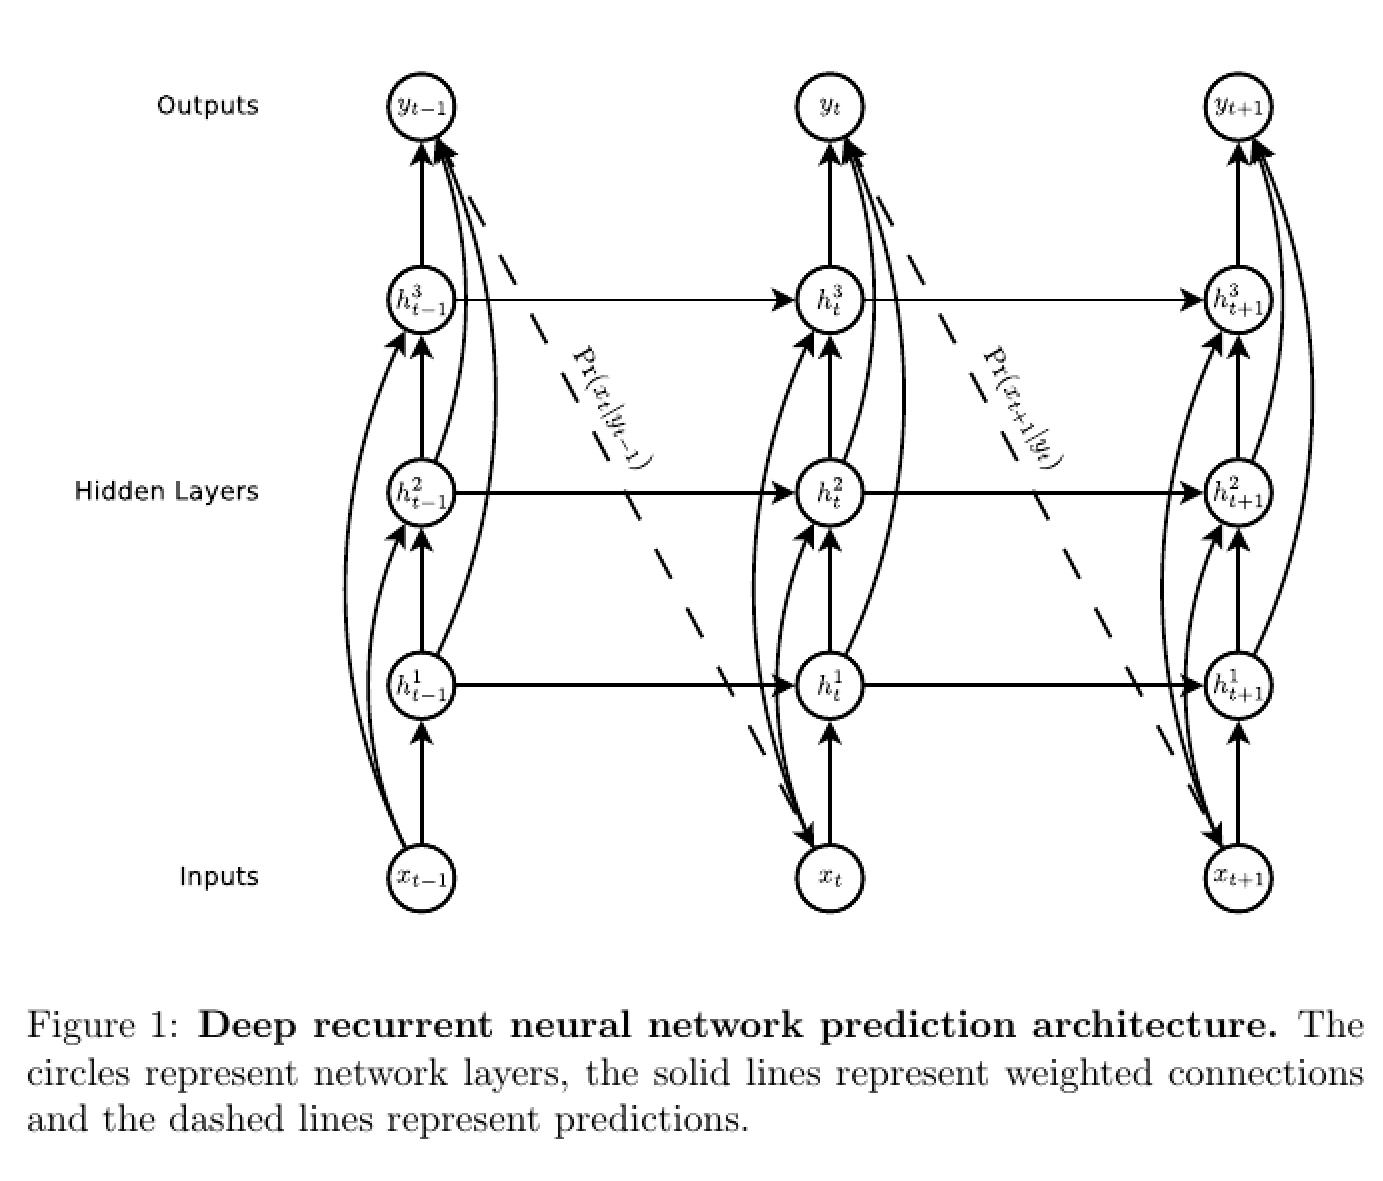
\includegraphics[width=.75\textwidth]{fig/figure1.png}
  \end{figure}
\end{frame}

\begin{frame}
  \begin{align*}
    \label{eq:eqs1-4}
    h_t^1 &= \cH(W_{ih^1} x_t + W_{h^1h^1} h_{t-1}^1 + b_h^1)  \\
    h_t^n &= \cH(W_{ih^n} x_t + W_{h^{n-1}h^{n}} h_{t}^{n-1} + W_{h^{n}h^{n}} h_{t-1}^n + b_h^n) \\
    \hat{y}_t &= b_y + \sum_{i=1}^N W_{h^n y}h_t^n \\
    y_t &= \cY(\hat{y}_t)
  \end{align*}

  Likelihood of input, loss function:
  \begin{align*}
    \bbP(\bfx) &= \prod_{t=1}^T \bbP(x_{t+1} \mid y_t) \\
    \cL(\bfx) &= -\sum_{t=1}^T \log \bbP(x_{t+1} \mid y_t)
  \end{align*}
\end{frame}


\begin{frame}{LSTM}
  \begin{figure}
    \centering
  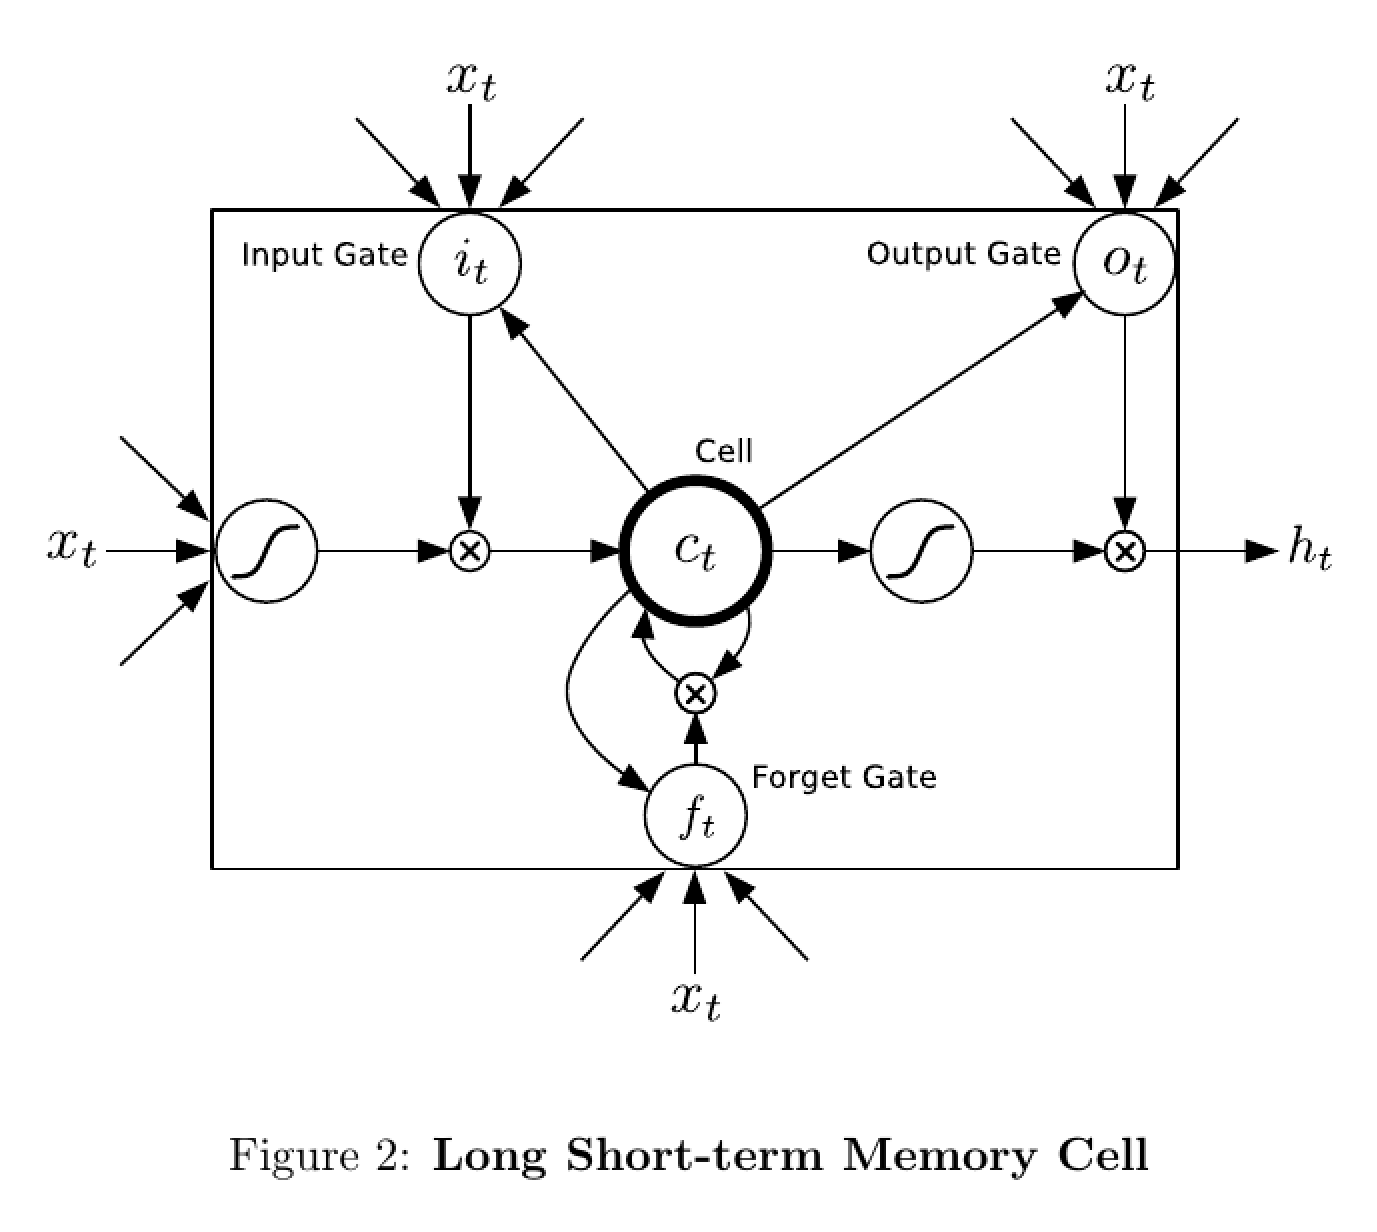
\includegraphics[width=.75\linewidth]{fig/figure2.png} 
  \end{figure}
\end{frame}

\begin{frame}
  Instead of 
  \begin{align*}
  h_t^n &= \cH(W_{ih^n} x_t + W_{h^{n-1}h^{n}} h_{t}^{n-1} + W_{h^{n}h^{n}} h_{t-1}^n + b_h^n)
  \end{align*}
  do we have instead the following?
  \begin{align*}
  h_t^n, c_t^n &= \cH(x_t, c_t^{n-1}, h_{t}^{n-1}, h_{t-1}^n)
  \end{align*}
\end{frame}

\begin{frame}
 For a really nice explanation of LSTM see:  

 \url{colah.github.io/posts/2015-08-Understanding-LSTMs}
\begin{columns}
  \begin{column}{.75\textwidth}
 \begin{figure}
   \centering
   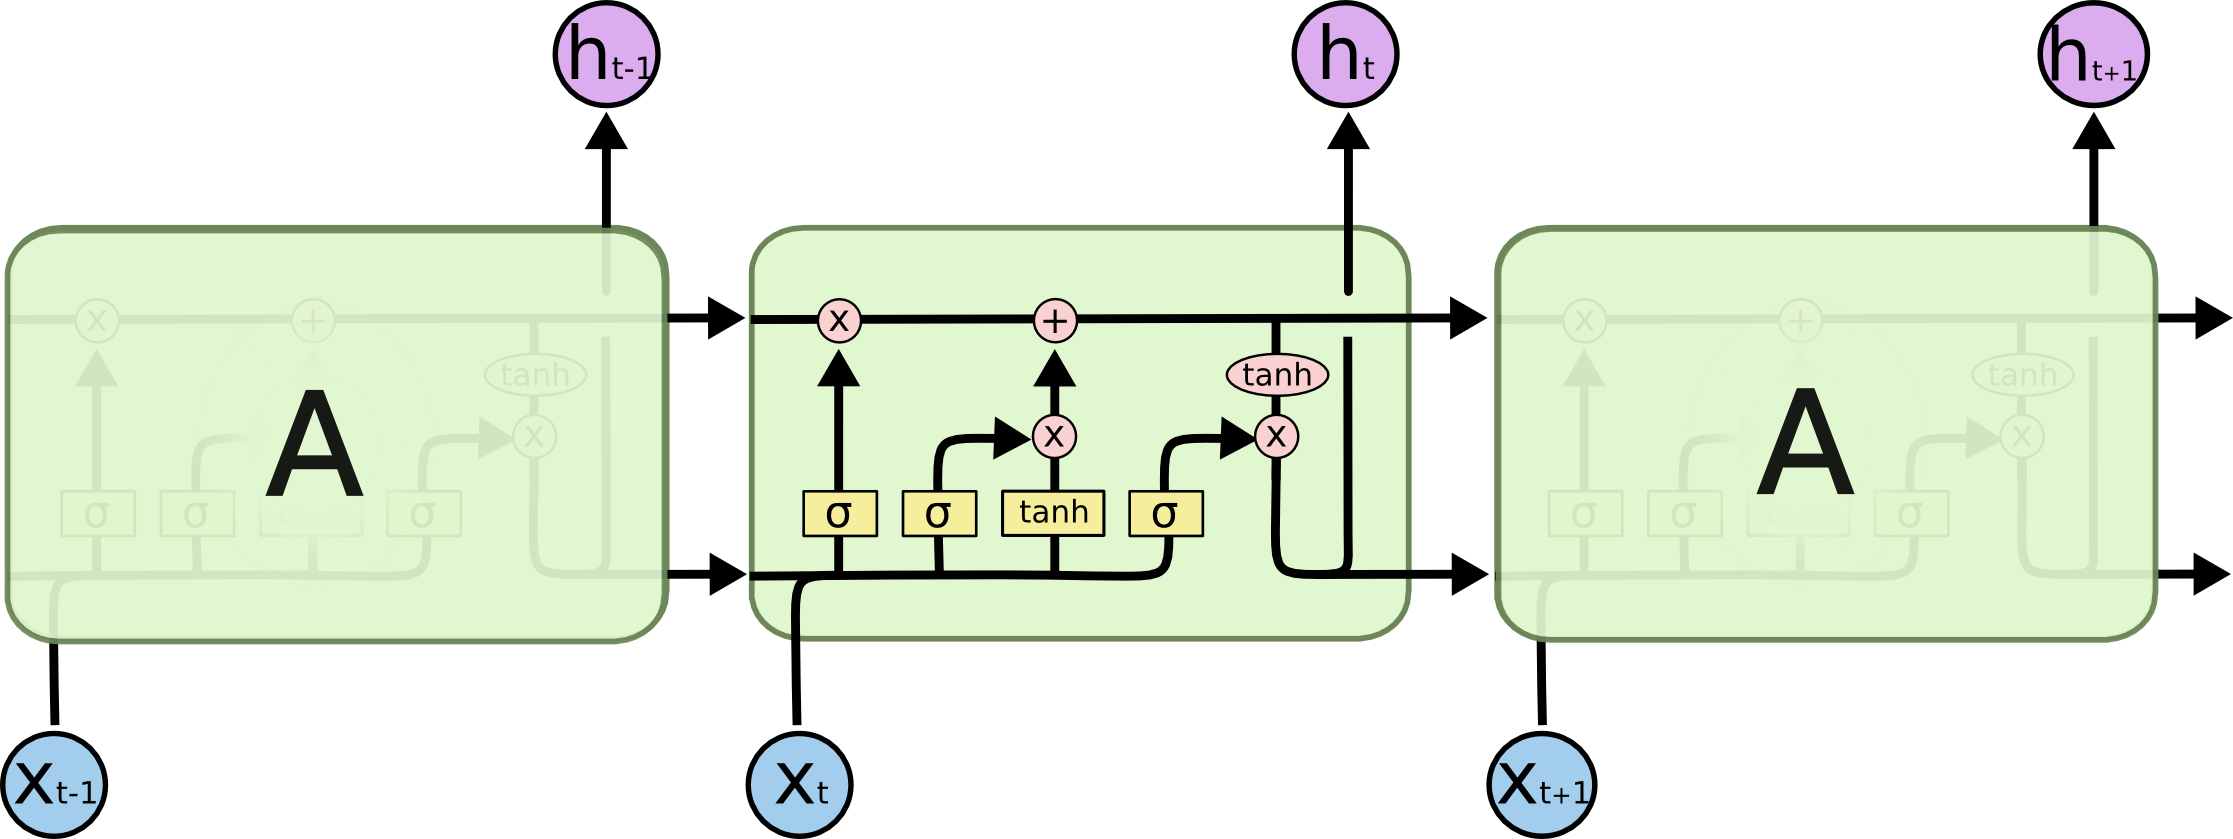
\includegraphics[width=\linewidth]{fig/LSTM3-chain.png} 
 \end{figure}
  \end{column}

  \begin{column}{.25\textwidth}
    \begin{block}{Gate=sigmoid + multiplication}
      \begin{figure}
        \centering
        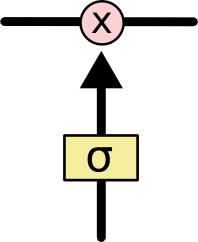
\includegraphics[width=.5\linewidth]{fig/LSTM3-gate.png} 
        \label{fig:gate}
      \end{figure}
\small{0='nothing thru' \\ 1='all thru'}
    \end{block}
  \end{column}
\end{columns}
\end{frame}


\begin{frame}
  \begin{overlayarea}{\textwidth}{.6\textheight}
    \begin{center}
      \only<1>{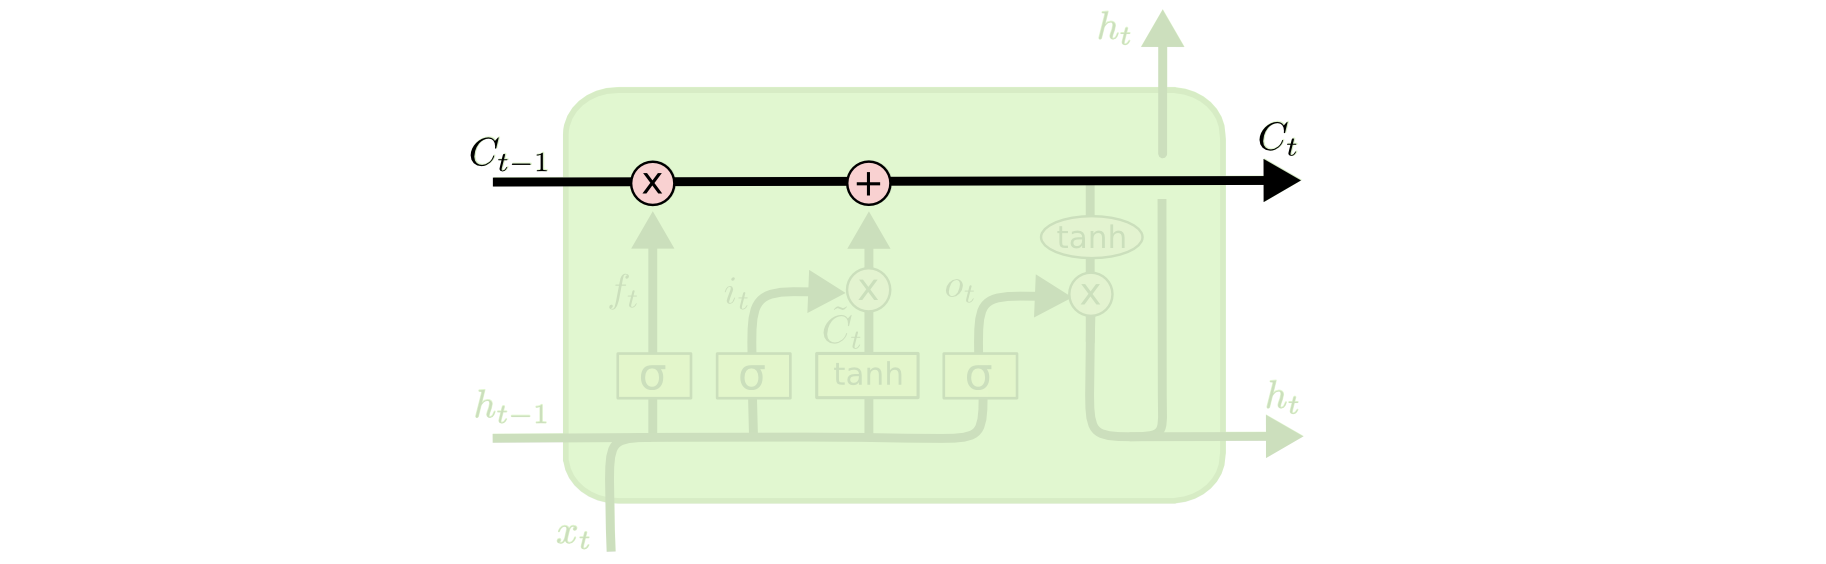
\includegraphics[width=\linewidth]{fig/LSTM3-C-line.png}} 
      \only<2>{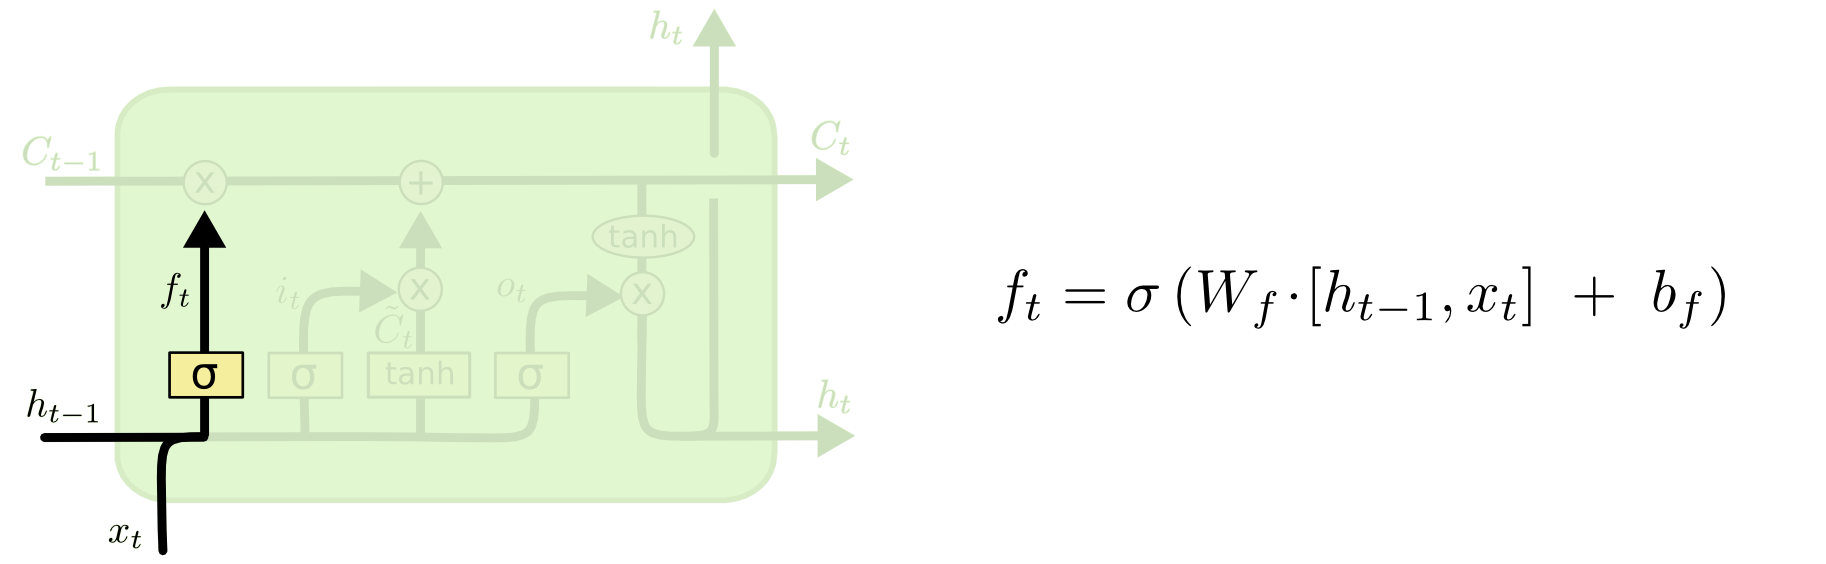
\includegraphics[width=\linewidth]{fig/LSTM3-focus-f.png}} 
      \only<3>{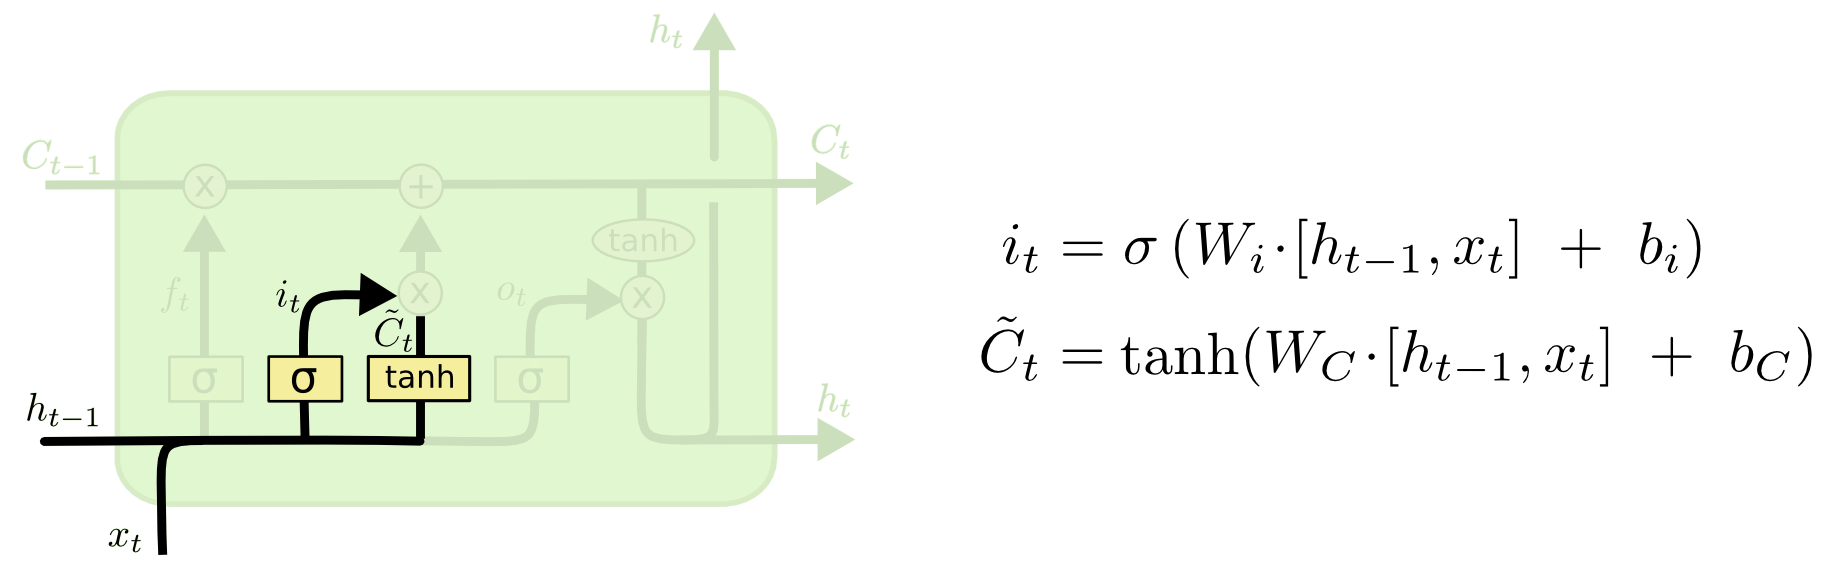
\includegraphics[width=\linewidth]{fig/LSTM3-focus-i.png}} 
      \only<4>{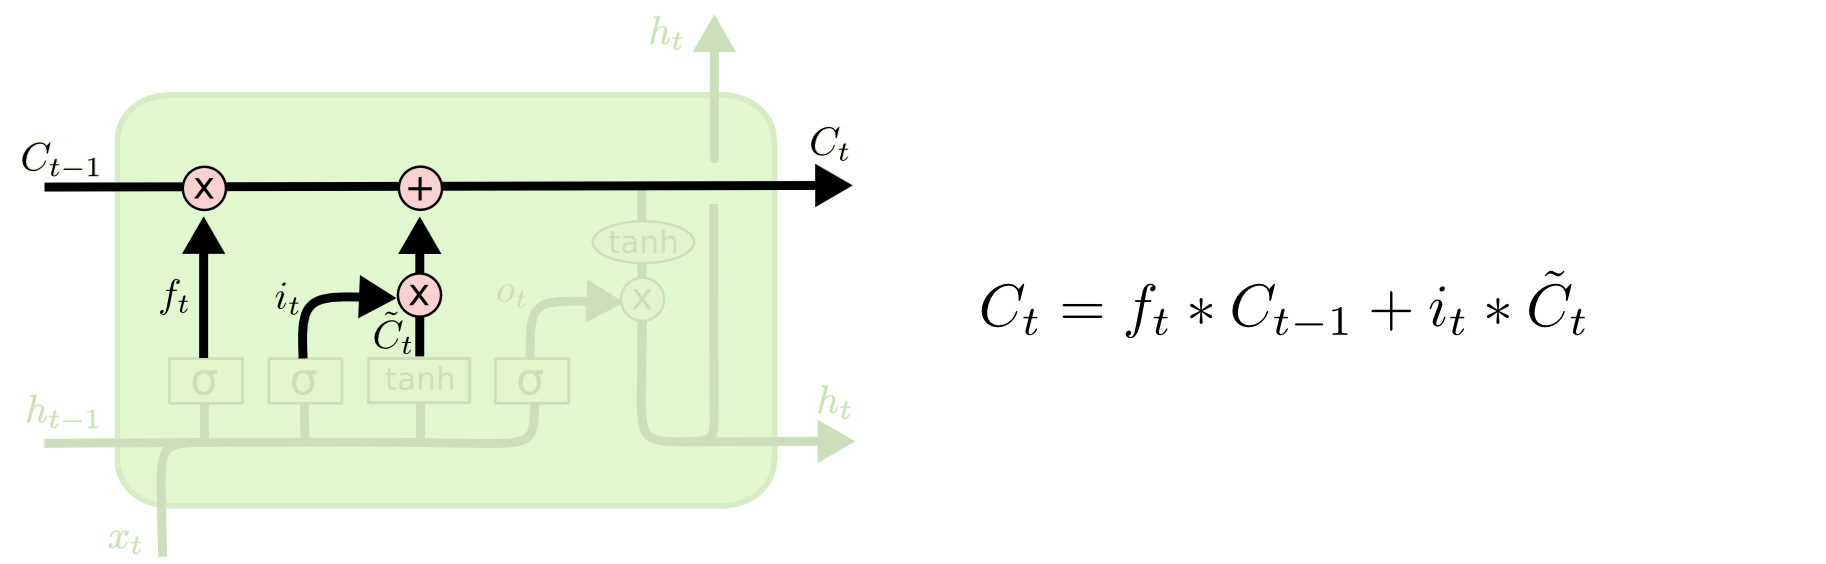
\includegraphics[width=\linewidth]{fig/LSTM3-focus-C.png}} 
      \only<5>{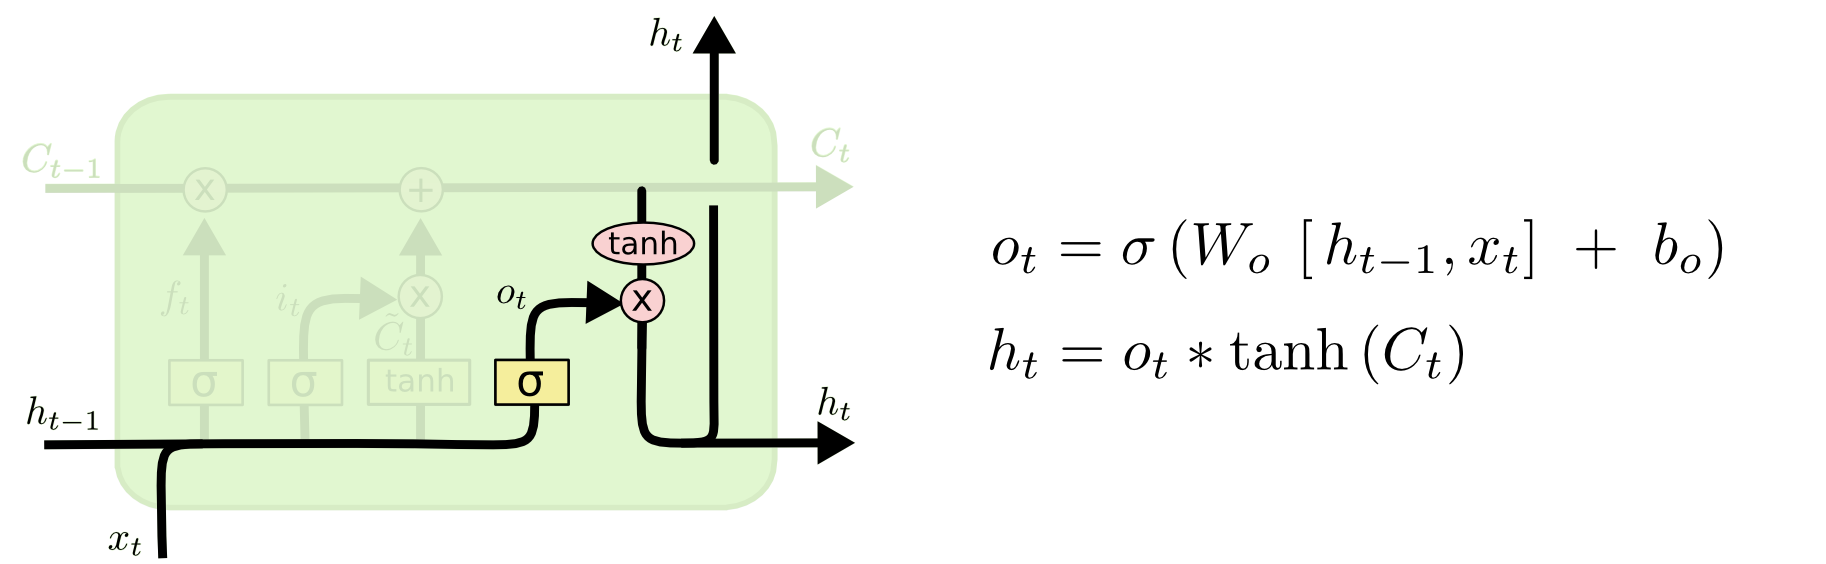
\includegraphics[width=\linewidth]{fig/LSTM3-focus-o.png}} 
    \end{center}
  \end{overlayarea}
  \only<1>{Information flows along cell state}
  \only<2>{Forget gate controls what to keep from previous}
  \only<3>{Input gate controls what to add from input}
  \only<4>{Update cell state from forget and input gates}
  \only<5>{Output gate controls what to output from cell state}
\end{frame}

\begin{frame}{Backpropagation thru time}
  \begin{itemize}
  \item Train with ``backpropagation thru time''
    \begin{itemize}
    \item Turn head sideways and do backpropagation
    \item i.e. reverse-mode automatic differentiation
    \end{itemize}
  \item Truncated backpropagation thru time
    \begin{itemize}
    \item Improve numerical stability by truncating gradients if they get too
      big as we go backwards thru the sequence
    \end{itemize}
  \end{itemize}
  Reference other papers?
\end{frame}

\section{Generating text}

\begin{frame}{Text Prediction}
  Basic framework for text prediction

  $y_t = \bbP(x_{t+1})$
  
  Per-character vs per-word prediction
\end{frame}

\begin{frame}{Penn Treebank Test Set}
  Penn Treebank
  
  Perplexity? BPC?

  Regularization schemes
\end{frame}

\begin{frame}{Wikipedia Experiments}
  \begin{itemize}
  \item   Wikipedia experiments
  \item \url{karpathy.github.io/2015/05/21/rnn-effectiveness} has some nice
    visualizations for understanding what's going on, e.g. what the inner
    neurons represent
  \end{itemize}
\end{frame}

\section{Generating handwriting}

\begin{frame}{Handwriting experiments}
  \begin{itemize}
  \item 
 Handwriting experiments 
 \item
 Mixture density outputs
 \begin{itemize}
 \item Basic framework for real valued outputs
 \end{itemize}
\item 
 Figure 10 is cool
  \end{itemize}
\end{frame}

\begin{frame}{Handwriting Synthesis}
 \begin{itemize}
 \item 
 Handwriting synthesis 
 \item Input, output sequences have different lengths
 \item Biased vs unbiased vs primed sampling
 \end{itemize}
\end{frame}




\end{document}
